\documentclass[10pt,twocolumn]{article}
\usepackage[a4paper,margin=1.8cm]{geometry}
\usepackage{graphicx,amsmath,amssymb,booktabs,xcolor}
\usepackage[hidelinks]{hyperref}
\usepackage[numbers,sort&compress]{natbib}
\setlength{\bibsep}{0pt}
\setlength{\abovecaptionskip}{5pt}
\graphicspath{{figures/}}
\newcommand{\ci}[2]{{\scriptsize[#1,\,#2]}}

\title{\vspace{-3ex}Is Optical Flow Needed for Stable Sketch Flipbooks?\\A Controlled Study of Frame-to-Frame Stroke Propagation}
\author{Rona Lavi, Ron Libman, Yamit Ehrlich, Sophie Danilov \\ Modern Computer Vision, Technion \\ \small\url{https://github.com/LaviRona/FlipBook}}
\date{\vspace{-5ex}}

\begin{document}
\maketitle

\begin{abstract}
A flipbook made from a video should resemble the video on every page and should not flicker when its pages are
flipped. CLIPasso draws a good sketch of a single image with a few strokes, but when every frame of a video is drawn
separately, the strokes jump from page to page. A natural remedy is to draw the frames in order, starting each drawing
from the previous one after moving its strokes along the optical flow. A recent video sketching method set optical flow
aside, warning that its errors might accumulate, without testing it. We build such a method one component at a time,
choose all settings on one clip, and evaluate on three new clips. Starting from the previous drawing turns out to
matter far more than following the optical flow.
\end{abstract}

\section{Introduction}
Our goal is to turn a short video into a flipbook: a small book of simple line drawings that shows the motion when its
pages are flipped. Each page should look like its video frame, and consecutive pages should differ only as much as the
object moves; when strokes move for no reason, the flipbook flickers. CLIPasso~\citep{vinker2022clipasso} draws a
recognizable sketch of an image with a few curved strokes, but run on each frame separately it starts every page from
a new random position, so the strokes jump between pages (Fig.~\ref{fig:onion}, top).

Recent video sketching methods reduce flicker by optimizing the drawings of all frames
together~\citep{zheng2024sketchvideo,fang2025video,zhu2025vector,zhu2026hypersketch}. A simpler approach is to draw the
frames in order and start each drawing from the previous one, after moving its strokes along the \emph{optical flow},
the estimated motion of every pixel between two frames. Earlier work disagrees on whether this helps. In painterly
rendering, strokes moved this way~\citep{litwinowicz1997processing,hertzmann2000painterly} flicker because motion errors
accumulate~\citep{collomosse2004mid}, while in video style transfer a flow-warped start works much better than an
unwarped one~\citep{ruder2016artistic}. For sketches, Zheng et al.~\citep{zheng2024sketchvideo} set optical flow aside
as ``the most naive approach'', warning of ``cumulative errors'', without testing it, and LiveSVG~\citep{levy2026livesvg}
finds that starting each vector frame from tracked points helps. To our knowledge, these starting points have not been
compared in a controlled study for CLIP-optimized line sketches.

We compare three ways of drawing the next frame (Fig.~\ref{fig:methods}). \emph{Per-frame} drawing runs CLIPasso from a
new random start. A \emph{warm start} begins from the finished drawing of the previous frame and adjusts it briefly.
\emph{Flow propagation}, our proposed method, first moves the previous drawing along the optical flow and then adjusts
it. We find that the warm start removes much of the flicker, that optical flow does not improve on it, and that errors
build up when strokes are tied to a predicted position but not with the plain warm start.

\begin{figure}[t]\centering
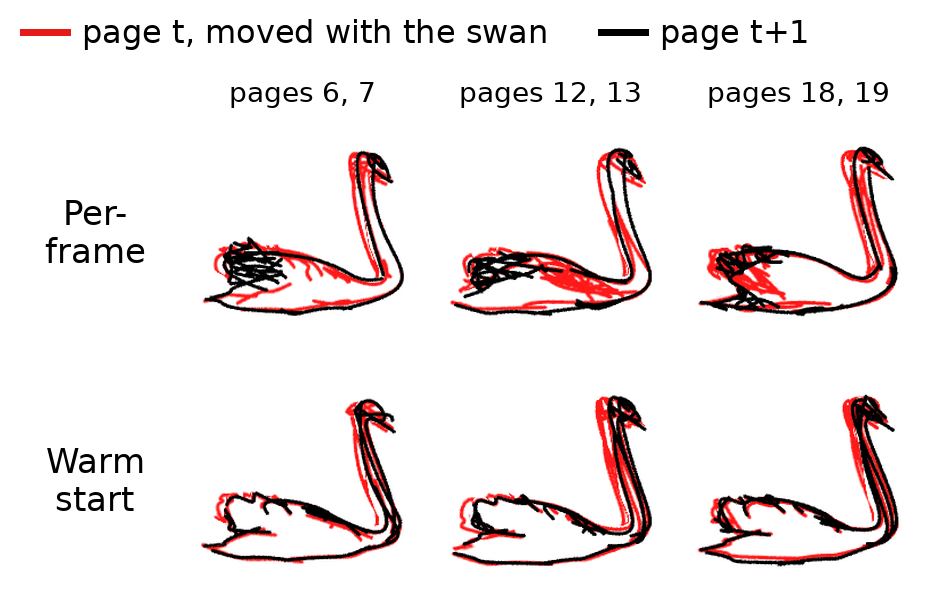
\includegraphics[width=0.95\linewidth]{fig_onion.png}
\caption{Flicker. Each image overlays two consecutive pages of the \emph{blackswan} flipbook: page $t$ in red,
shifted to follow the swan's own motion, and page $t{+}1$ in black. Where the strokes only moved with the swan, red and
black coincide. Drawing every page from scratch (top) redraws the body on every page; the warm start (bottom) keeps
it.}
\label{fig:onion}
\end{figure}

\section{Background}
\textbf{CLIPasso.} In our study a sketch has 16 strokes, each a cubic B\'ezier curve defined by four control points.
CLIPasso places the strokes at random positions drawn from a saliency map and then adjusts the control points by
gradient descent for about 2{,}000 steps (iterations), so that the drawing and the image look alike to
CLIP~\citep{radford2021clip}, a network trained to match images with text. A differentiable
rasterizer~\citep{li2020diffvg} passes the gradients from the image back to the control points. Because the
optimization has many local optima, different random starts give different drawings.

\textbf{Optical flow.} We estimate optical flow with RAFT~\citep{teed2020raft}. The flow is unreliable at
\emph{occlusions}, pixels that are visible in one frame but hidden in the next. We find them with a forward--backward
check~\citep{sundaram2010dense}: following the flow forward and back should return to the starting pixel.

\section{Methods}
All methods draw the first frame with CLIPasso and the remaining frames in order. They differ in how each new drawing
starts (Fig.~\ref{fig:methods}) and in a few additional steps.

\begin{figure}[t]\centering
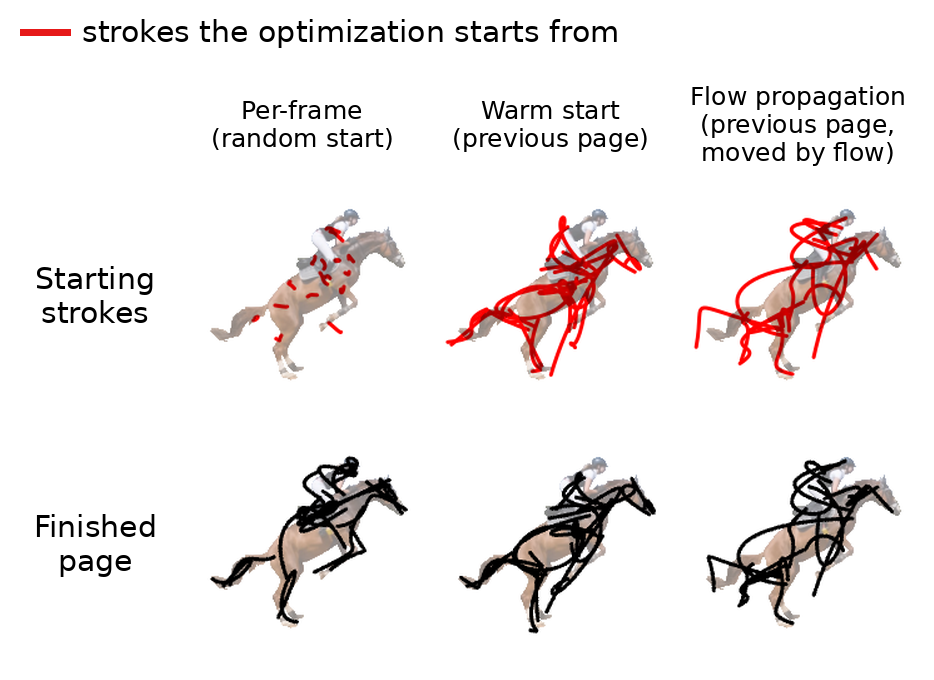
\includegraphics[width=\linewidth]{fig_methods.png}
\caption{How each method draws a new page (\emph{horsejump-high}, page 3). Top: the strokes the optimization
starts from (red), over the faded video frame. Bottom: the finished page. The warm start begins from page 2, which
lags behind the jumping horse; flow propagation begins from page 2 moved along the optical flow.}
\label{fig:methods}
\end{figure}

\textbf{Per-frame} drawing runs CLIPasso from scratch for 2{,}001 iterations, with one random start instead of the best
of three used by CLIPasso. The \textbf{warm start} continues the optimization from the previous drawing for only 150
iterations; in optimization, a warm start means starting from an earlier solution.

\textbf{Flow propagation} adds four steps to the warm start. (1)~The \emph{flow move} shifts each control point by the
optical flow at its position. (2)~\emph{Re-initialization} places strokes that lie mostly on occluded pixels again on
salient parts of the new frame. (3)~A \emph{regularizer} with weight $\lambda$ keeps the control points close to where
the flow moved them. (4)~Every $K$ frames, a \emph{keyframe} is refined for 500 iterations without the regularizer, to
correct accumulated errors.

Two variants isolate the flow. \textbf{Propagation without flow} is the same method without the flow move.
\textbf{Warm start + flow} is the warm start with only the flow move; we added it after seeing the test results.

\section{Experimental setup}
\textbf{Data.} We use 24-frame clips from DAVIS 2017~\citep{pont2017davis} (every second frame), cropped around the
object, resized to $224\times224$ pixels and placed on white. The \emph{dog} clip, with fast motion (10 pixels per
frame), is used only to choose settings. The test clips are \emph{blackswan} and \emph{camel}, which move slowly (2--3
pixels per frame), and \emph{horsejump-high} (7 pixels per frame, with a quarter of the horse occluded between frames).

\textbf{Measures.} \emph{Flicker} is how far the strokes move beyond the motion of the object: we shift drawing $t$ by
the video's motion to frame $t{+}1$ and measure the average distance to the nearest stroke pixel of drawing $t{+}1$,
in both directions (the chamfer distance). The shift uses a second flow model, GMFlow~\citep{xu2022gmflow,xu2023unifying},
so the measure does not favour methods that use RAFT. \emph{Fidelity} is how much a drawing resembles its frame,
measured by LPIPS~\citep{zhang2018lpips} (lower is closer) and CLIP ViT-L/14 similarity (higher is closer), a CLIP
model that CLIPasso does not use in its loss. \emph{Cost} is iterations per frame. All measures are relative to
per-frame drawing, so it scores 1.00.

\textbf{Protocol.} Each method runs with three random seeds per test clip; we report means over the nine runs with 95\%
bootstrap intervals. We chose $\lambda$ and $K$ on \emph{dog} only, taking the setting with the lowest flicker
whose LPIPS stayed within 10\% and CLIP similarity within 5\% of per-frame drawing ($\lambda{=}1.6{\cdot}10^{-3}$ with
flow, $\lambda{=}0$ without, $K{=}6$). On \emph{dog}, flow propagation was the best method. We then ran all methods
on the test clips without changing any setting.

\begin{table}[t]\centering\footnotesize
\caption{Results on the test clips, relative to per-frame drawing (mean of 9 runs; 95\% interval for flicker).
Iterations are per frame after the first. $^\dagger$Added after the test results.}
\label{tab:main}
\setlength{\tabcolsep}{2.3pt}
\begin{tabular}{@{}lcccr@{}}
\toprule
Method & Flicker $\downarrow$ & LPIPS $\downarrow$ & CLIP $\uparrow$ & Iter. \\
\midrule
Per-frame (CLIPasso) & 1.00 & 1.00 & 1.00 & 2001 \\
Per-frame, stopped early & 2.28 \ci{2.11}{2.48} & 1.25 & 0.90 & 150 \\
Warm start & \textbf{0.57} \ci{0.44}{0.72} & \textbf{1.04} & 0.99 & 150 \\
Propagation w/o flow & 0.82 \ci{0.62}{1.04} & 1.08 & 1.00 & 196 \\
Flow propagation (ours) & 0.83 \ci{0.54}{1.19} & 1.38 & 0.96 & 196 \\
\midrule
Warm start + flow$^\dagger$ & 0.58 \ci{0.44}{0.75} & 1.29 & 0.98 & 150 \\
\bottomrule
\end{tabular}
\end{table}

\begin{figure}[t]\centering
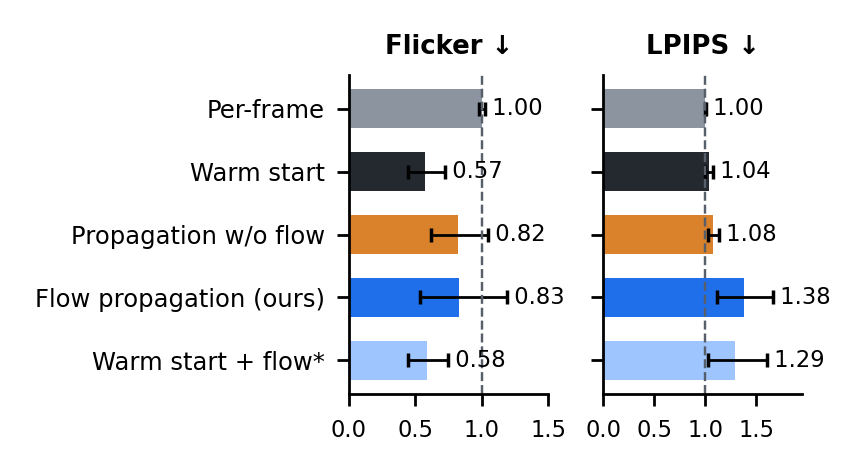
\includegraphics[width=\linewidth]{overview.png}
\caption{Flicker (left) and LPIPS (right) on the three test clips, relative to drawing every page from scratch
(dashed line); lower is better for both. Bars are means of 9 runs; whiskers are 95\% intervals. *Added after the
test results.}
\label{fig:overview}
\end{figure}

\section{Results}
\textbf{The warm start performs best} (Table~\ref{tab:main}, Fig.~\ref{fig:overview}). It reduces flicker by 43\% at
almost the same fidelity, with 13 times fewer iterations per frame. The gain comes from the starting point, not from
the shorter optimization: per-frame drawing stopped after the same 150 iterations flickers four times as much. The 95\%
interval of the reduction is 28--56\%.

\textbf{Flow propagation does not do better.} It removes less flicker than the warm start, about as much as
propagation without flow, and it is the least faithful method (LPIPS 1.38). Re-initialization and keyframes also add some flicker of their own
compared with the plain warm start, although the intervals overlap.

\begin{figure}[t]\centering
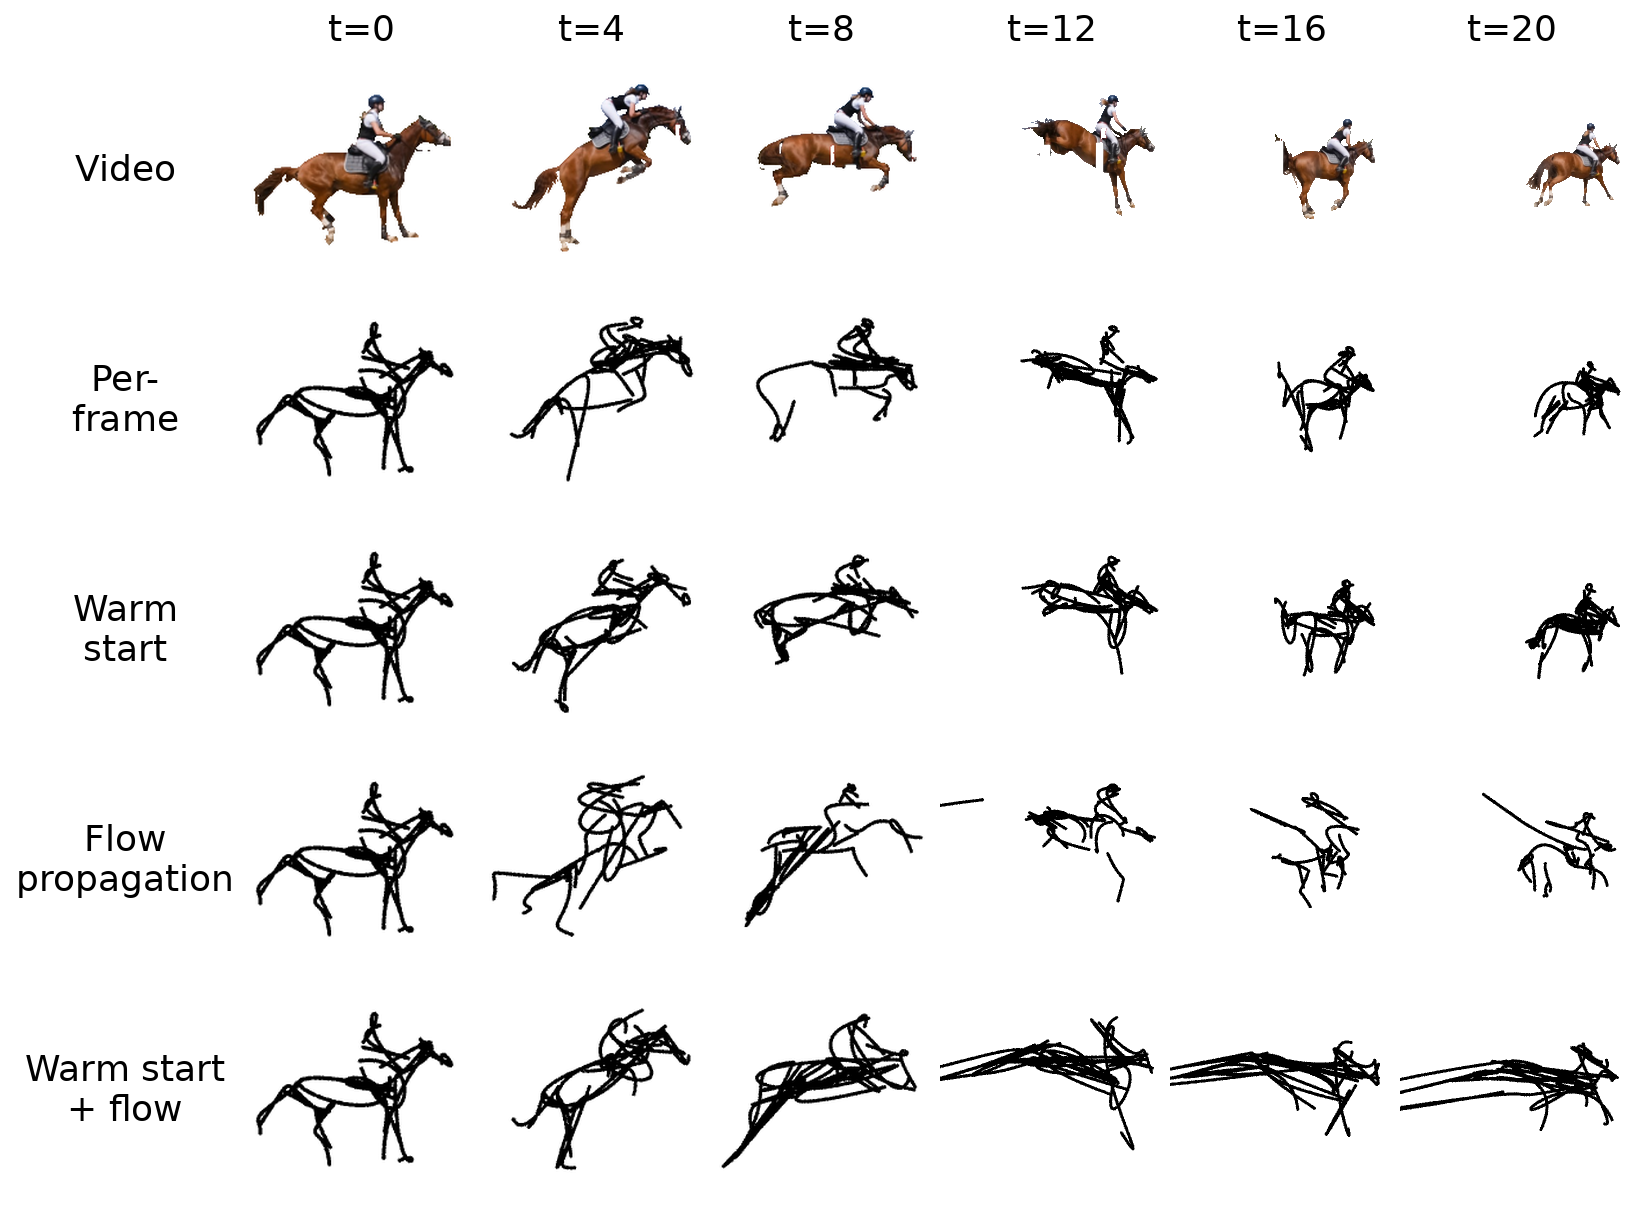
\includegraphics[width=\linewidth]{fig_strip.png}
\caption{Pages of \emph{horsejump-high} (columns) for each method (rows). Once the horse jumps, the two methods
that move strokes with the optical flow stretch them across the page.}
\label{fig:strip}
\end{figure}

\textbf{Does optical flow help?} Within the proposed method, yes: when both propagation methods use the same
$\lambda$, the flow move lowers flicker by up to 26\%. (Their chosen settings in Table~\ref{tab:main} use different
values of $\lambda$.) Compared with the plain warm start, no: adding the flow leaves flicker unchanged and lowers
fidelity. Fig.~\ref{fig:strip} shows why. When the horse jumps and is partly hidden, the flow is wrong for some control
points and the strokes are stretched across the page. The flow helped clearly only on the fast development clip.

\textbf{Do errors accumulate?} We track the difference between each method's LPIPS and that of per-frame drawing over
the 24 frames; if errors build up, this gap grows. With the plain warm start it stays flat. It grows when a
regularizer pulls the strokes toward a predicted position, faster for larger $\lambda$, and when the flow moves them.
Keyframes reset the gap, but it grows again afterwards. The cumulative errors that Zheng et al.\ warned about therefore
appear under these constraints, not with the plain warm start.

\section{Discussion}
For slow and moderate motion, a simple recipe works: start each drawing from the previous one and refine it briefly.
Following the optical flow adds complexity without a benefit on our test clips and fails under fast, occluded motion.
This differs from video style transfer~\citep{ruder2016artistic} and LiveSVG~\citep{levy2026livesvg}, where a
flow-warped or tracked start helped. A likely reason is that an image cannot follow the object without the flow,
whereas our 16 strokes can catch up with it during refinement. On the fast development clip, however, the warm start
alone did not reduce flicker, so faster motion may still need the flow.

\textbf{Limitations.} We chose the settings on a clip that moves faster than any test clip, which favoured the flow;
a development set with several motion sizes would be more reliable. We tested only three clips of 24 frames and did
not compare with a whole-video method. Full results are in the repository.

{\scriptsize
\bibliographystyle{abbrvnat}
\bibliography{refs}}
\end{document}
